
\section*{Executive Summary}
\addcontentsline{toc}{section}{Executive Summary}
\label{sec:execsum}

\begin{figure}
 %   \centering
    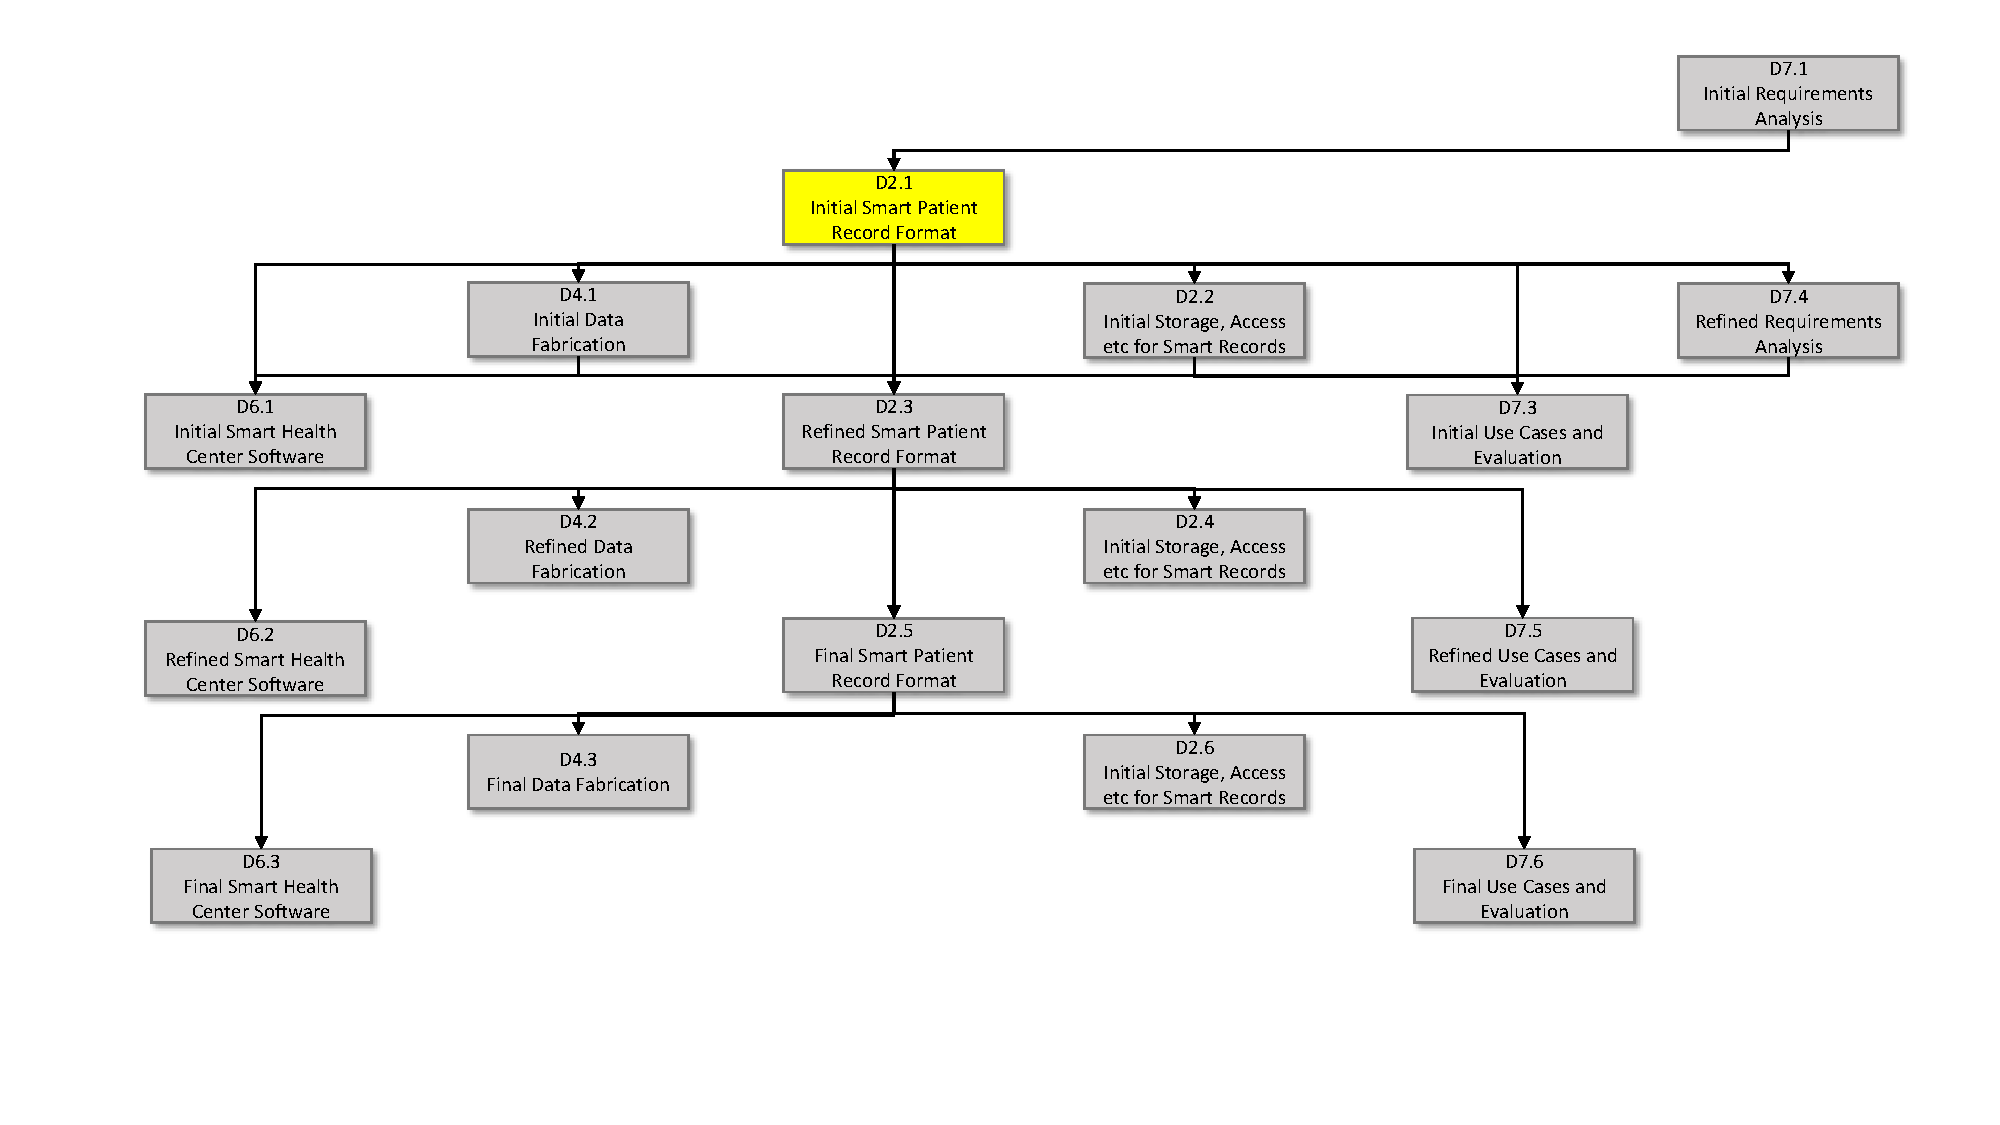
\includegraphics[scale=0.42]{figures/Serums-D21-Dependencies.pdf}
    \caption{Dependencies between D2.1 and other deliverables}
    \label{fig:WP2dependencies}
\end{figure}

This deliverable describes the initial version of the smart patient record format that will be used throughout the \textbf{Serums} project for encapsulating the patient data. It is a part of WP2, the objectives of which are to:
\begin{enumerate}
    \item define a format for smart patient records that can contain data distributed over multiple devices 
    \item develop mechanisms to track the lineage of accesses to the smart patient records
    \item to develop mechanisms to control storage and access rights for smart patient records
    \item to build on existing and develop new machine learning methods for extracting meta-data from unstructured data
\end{enumerate}

Precise specification of the format of the data that will be used in the project is crucial to many parts of the project, e.g.~for the development of the block-chain technology to track the access to this data (WP2), distributed privacy-preserving data analytics (WP3), data fabrication technology to generate synthetic but realistic data to be used in development and testing of the other technologies in the project (WP4) and use cases development (WP7). Therefore, the results of this deliverable will be used extensively in the other parts of the project. Figure~\ref{fig:WP2dependencies} shows the graph of the dependencies between this deliverable and other relevant deliverables in the project. 

In the subsequent deliverable related to the smart patient record format, we will extend the format presented in this deliverable to accommodate to the data that can reside on different sources within the same organisation (D2.3), as well as the data that might need to be collected/exchanged outside of the local environment, e.g.~in scenarios of trans-national exchange of data (D2.5).